 \providecommand{\main}{../../..}
\documentclass[\main/main.tex]{subfiles}
\begin{document}
\subsection{Esercizio 1}
Dato il seguente problema di PL:

\begin{figure}
  \begin{align*}
    \max z = -x_1 + 2x_2 \\
    x_1 + 2x_2 & \leq 12 \\
    x_1        & \leq 8  \\
    x_1 + x_2  & \geq 3  \\
    -x_1 + x_2 & \leq 3  \\
    x_1, x_2   & \geq 0
  \end{align*}
  \caption{Esercizio 1}
\end{figure}

\begin{enumerate}
  \item Si disegni la regione ammissibile e si evidenzi il vertice ottimo per via grafica, riportando il valore di z e di tutte le variabili del modello, comprese quelle di scarto.
  \item Da quali variabili è composta la base associata al vertice dato dall'intersezione del vincolo $\rom{3}$ e l'asse delle $x_1$?
  \item Si ricavi per via grafica per quali valori di $b_4$, ora pari a $3$, la \textbf{composizione} della base ottima non cambia.
  \item Si risolva mediante gli scarti complementari il duale del problema.
\end{enumerate}

\subsection{Soluzione esercizio 1}

\subsubsection*{Identifico soluzione ottima}

\begin{figure}
  \begin{subfigure}{0.49\textwidth}
    \dddgraph{x_1}{x_2}{0}{5}{-4}{5}{-17}{
      x + 2*y  <= 12 &&
      x        <= 8  &&
      x + y    >= 3  &&
      -x + y  <= 3}{-x +2*y}
    \caption{Il vertice ottimo ha coordinate $\bmx = \rnd{2,5}$}
  \end{subfigure}
  \begin{subfigure}{0.49\textwidth}
    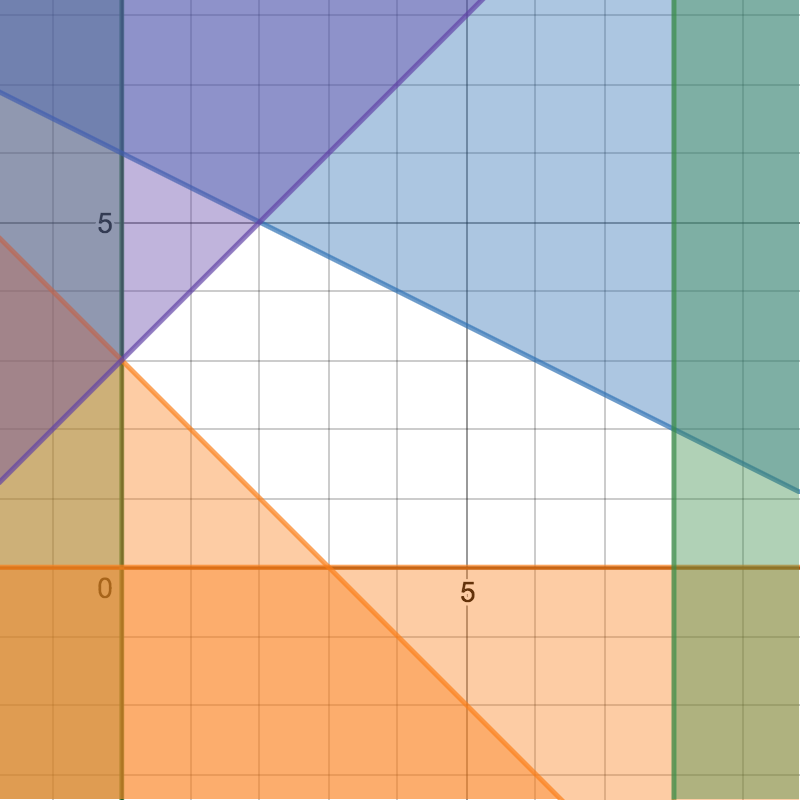
\includegraphics[width=0.9\textwidth]{2014_06_18}
    \caption{Regione di ammissibilità del problema}
  \end{subfigure}
  \caption{Vertice ottimo del problema di minimo}
\end{figure}

\subsubsection*{Riporto variabili}

\begin{align*}
  z = 8, \quad
  x_1 = 2, \quad
  x_2 = 5, \quad
  s_1 = 0, \quad
  s_2 = 6, \quad
  s_3 = 4, \quad
  s_4 = 0
\end{align*}
\subsubsection*{Composizione della base}
TODO: non so rispondere alla domanda.

\subsubsection*{Analisi di sensitività}
Posso variare $b_4$ tra $-3$ arrivando al vertice $(3,0)$ e $6$ al vertice $(0,6)$.

\begin{figure}
  \begin{subfigure}{0.49\textwidth}
    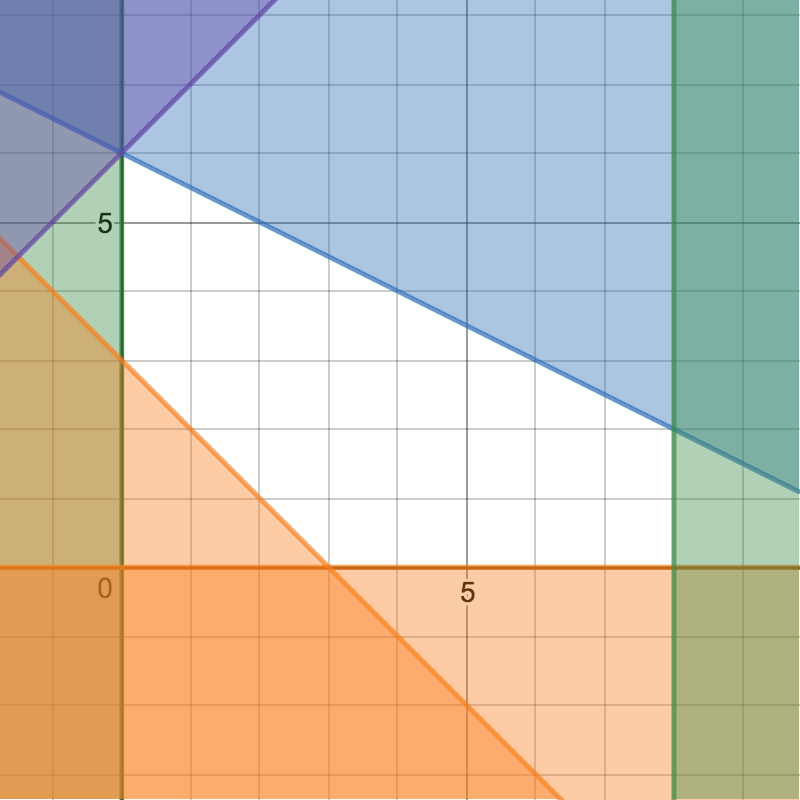
\includegraphics[width=0.9\textwidth]{2014_06_18_1}
    \caption{$b_4 = 6$}
  \end{subfigure}
  \begin{subfigure}{0.49\textwidth}
    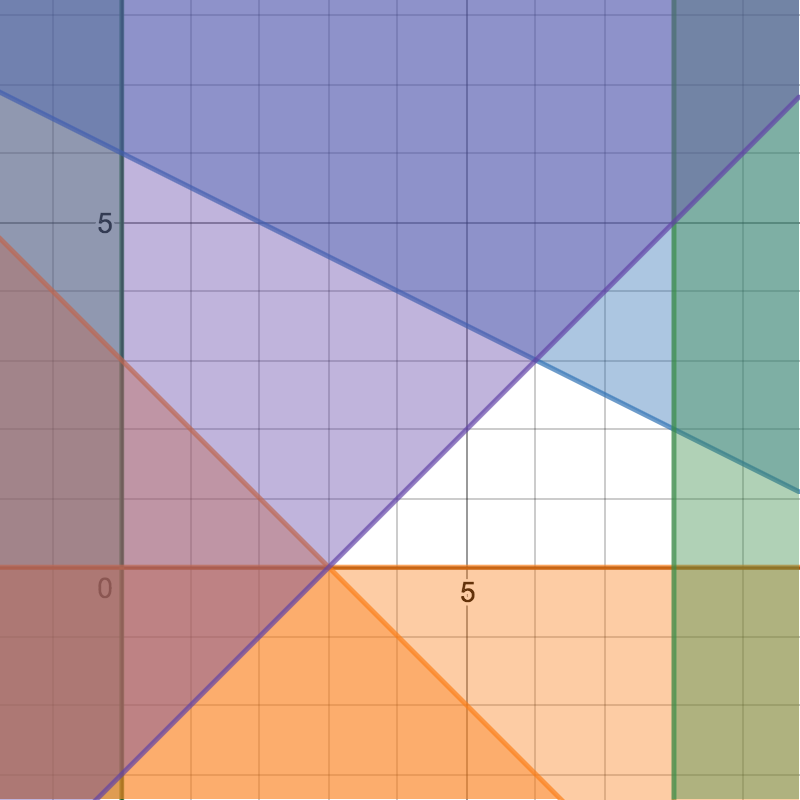
\includegraphics[width=0.9\textwidth]{2014_06_18_2}
    \caption{$b_4 = -3$}
  \end{subfigure}
  \caption{Analisi di sensitività}
\end{figure}

\subsubsection*{Costruisco problema duale}
\begin{align*}
  \min z_D = 12y_1 + 8y_2 + 3y_3 + 3y_4 \\
  y_1 + y_2 + y_3 -y_4 & \geq -1        \\
  2y_1 + y_3 + y_4     & \geq 2         \\
  y_1, y_2, y_4        & \geq 0         \\
  y_3                  & \leq 0
\end{align*}
\subsubsection*{Scarti complementari}
\[
  \begin{cases}
    x_1(y_1 + y_2 + y_3 -y_4 +1)=0  \\
    x_2(2y_1 + y_3 + y_4     -2 )=0 \\
    y_1(x_1 + 2x_2 -12)=0           \\
    y_2(x_1        -8 )=0           \\
    y_3(x_1 + x_2  -3 )=0           \\
    y_4(-x_1 + x_2 -3 )=0           \\
  \end{cases}
  \Rightarrow
  \begin{cases}
    y_1 -y_4 +1=0  \\
    2y_1 + y_4-2=0 \\
    y_2=0          \\
    y_3=0          \\
  \end{cases}
  \Rightarrow
  \begin{cases}
    y_1=\frac{1}{3} \\
    y_4=\frac{4}{3} \\
    y_2=0           \\
    y_3=0           \\
  \end{cases}
\]
La soluzione ottima del duale corrisponde a quella del primale: $z = z_D = 8$
\end{document}